
\documentclass{exam}

\usepackage{graphicx}
\usepackage[fleqn]{amsmath}
\usepackage{unitsdef} 
\usepackage{cancel}
\usepackage{float}
\usepackage{mdwlist}
\usepackage{booktabs}
\usepackage{cancel}
\usepackage{polynom}
\usepackage{caption}
\usepackage{fullpage}
\usepackage{enumerate}
\usepackage{parskip}

% \newcommand{\degree}{\ensuremath{^\circ}} 
\everymath{\displaystyle}

\newunit{\inch}{in}
\newunit{\foot}{ft}
\newunit{\cemtimeter}{cm}

% \begin{figure}[H]
%   \centering
%   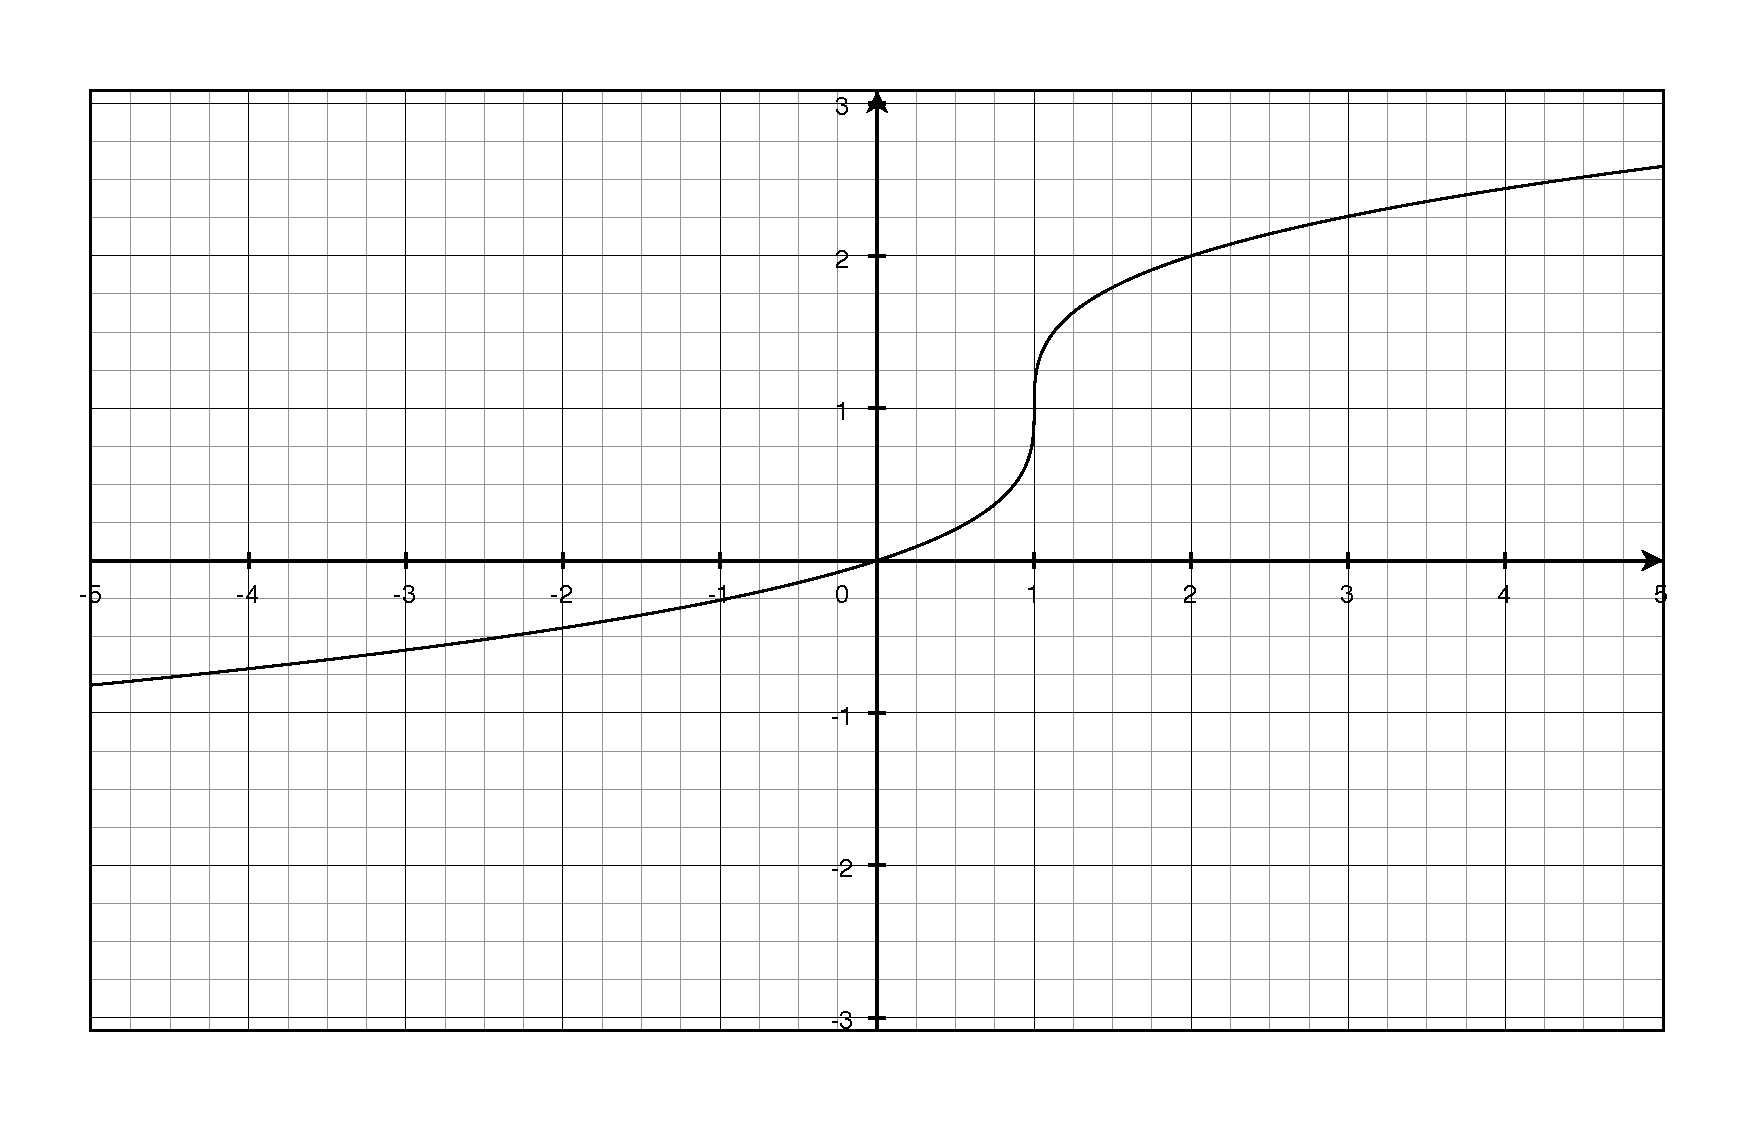
\includegraphics[scale=.3]{question7.eps}
%   \caption*{Question 7}
% \end{figure}

% \begin{tabular}{cc}
% \toprule
% period & amplitude \\
% \midrule
%   $\pi$ & $2$ \\
% \bottomrule
% \end{tabular}

\printanswers

\ifprintanswers 
\usepackage{2in1, lscape} 
\fi

\title{Math 263B \\ Homework Eight}
\date{September 13, 2012}

\begin{document}

\maketitle

\section{Homework}

\begin{itemize*}
  \item Read Section 6.2
  \item pp 310-312: 1-17, 23
\end{itemize*}

%% \ifprintanswers
%% \pagebreak
%% \fi

\section{Extra Credit}
page 312, problem 34

\ifprintanswers

\pagebreak

\begin{description}
\item[34]
Since we're rotating around the y axis, we need x as a function of y:
\begin{align*}
  y &= kx^4 \\
  x &= \left( \frac{y}{k} \right)^{1/4}
\end{align*}

If the height of the tank is $h$, the volume is:
\begin{align*}
  V &= \pi \int_0^h \left[ \left( \frac{y}{k} \right)^{1/4} \right]^2 \, \mathrm{d}y \\
  &= \pi \int_0^h \left( \frac{y}{k} \right)^{1/2} \, \mathrm{d}y \\
  &= \frac{\pi}{3} h^{3/2} \\
\end{align*}

Or, as a function of y: $V = \frac{2 \pi}{3 \sqrt{k}} y^{3/2}$

To calculate the derivative of the volume with respect to time, you need to use the chain rule, since y is also a function of time:
\[
  \frac{dV}{dt} = \frac{d}{dt} \left(\frac{2 \pi}{3 \sqrt{k}} y^{3/2} \right) = \frac{\pi}{\sqrt{k}} y^{1/2} \frac{dy}{dt}
\]

This has to be equal to the other expression for $\frac{dV}{dt}$.  When we set them equal to each other, the y's cancel out:
\begin{align*}
  \frac{\pi}{\sqrt{k}} \sqrt{y} \frac{dy}{dt} &= -m \sqrt{y} \\
  \frac{dy}{dt} &= - \frac{m}{\pi \sqrt{k}} \\
\end{align*}

The problem doesn't explain what $m$ is, but I think it is a constant related to the size of the hole in the tank and
the force of gravity.  Anyway, since there are no variables in the final expression, the water level falls at a constant rate.

\pagebreak

\uplevel{\section{Section 5.8}}

\item[1]
\[
  \pi \int_0^2 (x^2 + 1)^2 \, \mathrm{d}x = \frac{206 \pi}{15}
\]

\item[2]
\[
  \pi \int_0^3 (-x^2 + 4x)^2 \, \mathrm{d}x = \frac{153 \pi}{5}
\]

\item[3]
\begin{enumerate}[a]
\item
\[
  \pi \int_0^2 (4 - x^2)^2 \, \mathrm{d}x = \frac{256 \pi}{15}
\]

\item
solve for x in terms of y: $x = \sqrt{4 - y}$
\[
  \pi \int_0^4 (4 - y) \, \mathrm{d}y = 8 \pi
\]
\end{enumerate}

\item[4]
\begin{enumerate}[a]
\item
\[
  \pi \int_0^2 (4 - 2x)^2 \, \mathrm{d}x = \frac{32 \pi}{3}
\]

\item
solve for x in terms of y: $x = 2 - \frac{y}{2}$
\[
  \pi \int_0^4 \left( 2 - \frac{y}{2} \right)^2 \, \mathrm{d}y = \frac{16 \pi}{3}
\]

\end{enumerate}

\item[5]

\[
  \pi \int_0^4 \left( \frac{x^2}{\pi} \right)^2 \, \mathrm{d}x = \frac{1}{\pi} \int_0^4 x^4 \, \mathrm{d}x = \frac{1,024}{5 \pi}
\]

\item[6]
\[
  \pi \int_0^3 \left( x^3 \right)^2 \, \mathrm{d}x = \pi \int_0^3 x^6 \, \mathrm{d}x = \frac{2,187 \pi}{7}
\]

\item[7]
\[
  \pi \int_2^4 \left( \frac{1}{x} \right)^2 \, \mathrm{d}x = \pi \int_2^4 x^{-2} \, \mathrm{d}x = \frac{\pi}{4}
\]

\item[8]
\[
  \pi \int_2^3 \left( x^{3/2} \right)^2 \, \mathrm{d}x = \pi \int_2^3 x^3 \, \mathrm{d}x = \frac{65 \pi}{4}
\]

\item[9]
\[
  \pi \int_{-2}^3 \left( \sqrt{9 - x^2} \right)^2 \, \mathrm{d}x = \pi \int_{-2}^3 \left(9 - x^2 \right) \, \mathrm{d}x = \frac{100 \pi}{3}
\]

\item[10]
\[
  \pi \int_1^{27} \left( x^{2/3} \right)^2 \, \mathrm{d}x = \pi \int_1^{27} x^{4/3} \, \mathrm{d}x = \frac{6,558 \pi}{7}
\]

\item[11]
\[
  \pi \int_0^3 \left( y^2 \right)^2 \, \mathrm{d}y = \pi \int_0^3 y^4 \, \mathrm{d}y = \frac{243 \pi}{5}
\]

\item[12]
\[
  \pi \int_2^6 \left( \frac{2}{y} \right)^2 \, \mathrm{d}y = \pi \int_2^6 4y^{-2} \, \mathrm{d}y = \frac{4 \pi}{3}
\]

\item[13]
\[
  \pi \int_0^4 \left( 2 \sqrt{y} \right)^2 \, \mathrm{d}y = \pi \int_0^4 4y \, \mathrm{d}y = 32 \pi
\]

\item[14]
\[
  \pi \int_0^{27} \left( y^{2/3} \right)^2 \, \mathrm{d}y = \pi \int_0^{27} y^{4/3} \, \mathrm{d}y = \frac{6,561 \pi}{7}
\]

\item[15]
\[
  \pi \int_0^9 \left( y^{3/2} \right)^2 \, \mathrm{d}y = \pi \int_0^9 y^3 \, \mathrm{d}y = \frac{6,561 \pi}{4}
\]

\item[16]
\[
  2 \pi \int_0^2 \left( \sqrt{4 - y^2} \right)^2 \, \mathrm{d}y = 2 \pi \int_0^2 (4 - y^2) \, \mathrm{d}y = \frac{32 \pi}{3}
\]

\item[17]
Solve the equation for y:
\begin{align*}
  \frac{x^2}{a^2} + \frac{y^2}{b^2} &= 1 \\
  y &= \sqrt{b^2 - \frac{b^2x^2}{a^2}} \\
\end{align*}

Since the figure is symmetric, it's easiest to find half the volume and then multiply by 2:
\begin{align*}
  2 \pi \int_0^a \left( \sqrt{b^2 - \frac{b^2x^2}{a^2}} \right)^2 \, \mathrm{d}x 
    &= 2 \pi \int_0^a \left( b^2 - \frac{b^2x^2}{a^2} \right) \, \mathrm{d}x \\
    &= 2 \pi b^2 \int_0^a \left(1 - \frac{x^2}{a^2} \right) \, \mathrm{d}x \\
    &= 2 \pi b^2 \left(x - \frac{x^3}{3a^2} \right) \bigg|_0^a \\
    &= \frac{4 \pi a b^2}{3} \\
\end{align*}

Notice that if $a = b$ you have a sphere with radius $a$ and the formula reduces to $\frac{4 \pi a^3}{3}$ which is the
correct formula for the volume of a sphere.

\item[23]

First solve the equation for y in terms of x.  This gives the length of the side of each square slice.
\begin{align*}
  x^2 + y^2 &= 4 \\
  y &= \sqrt{4 - x^2} \\
\end{align*}

The volume of a slice is
\[
  V_{slice} = \left( 2 \sqrt{4 - x^2} \right)^2 \, dx = 4(4 - x^2) \, dx
\]

It's easiest to calculate half the volume and multiply by 2:
\[
  V = 2 \int_0^2 4(4 - x^2) \, \mathrm{d}x = \frac{128}{3}
\]
\end{description}

\else

\vspace{10 cm}

The most effective way to restrict democracy is to transfer decision-making from the public arena to unaccountable
institutions: kings and princes, priestly castes, military juntas, party dictatorships, or modern corporations.

\hspace{0.5 cm} 

--Noam Chomsky

%% {\em Some writers have so confounded society with government, as to leave little or no distinction between them; whereas
%%   they are not only different, but have different origins. Society is produced by our wants, and government by our
%%   wickedness; the former promotes our happiness POSITIVELY by uniting our affections, the latter NEGATIVELY by
%%   restraining our vices. The one encourages intercourse, the other creates distinctions. The first a patron, the last a
%%   punisher.} --Thomas Paine

\fi

\end{document}

